\documentclass{jlreq}
\usepackage{graphicx}
\usepackage{url}
\usepackage{booktabs, colortbl}
% \usepackage{hyperref}
% \usepackage{pxjahyper}

\title{第3回レポート \\ \vspace{0.4cm} ネットワーク構築}
\author{1270381 宮本武}
\date{2024年12月3日}

\begin{document}

\maketitle

\section{目的}
% ・内容がないと発生する不都合や問題(背景)\\

インターネットは私たちにとって一つの重要なインフラである.
インターネットを構成している単位はLANと呼ばれるネットワークである.
私たちがインターネットを利用するためには,このLANを単位とした一つのネットワークを構築する必要がある.
ある程度大きなネットワークを構築する際には,使用するネットワークを適切に分割することが重要である.

% ・内容をすることで何ができるようになるのか(目的)\\

ネットワークの分割には以下のようなメリットがある.

\begin{description}
    \item [効率性の向上] ネットワークの把握,管理が容易になる点,通信におけるネットワーク機器の負担を分散させられる点などが挙げられる.
    ネットワークの構造を把握しやすければ,ネットワーク障害が発生したとしても,原因の究明を迅速に行うことができる.
    そして,障害を限定させることで,復旧作業の効率化を図ることができる.
    また,ネットワークを分割してセグメントごとに通信経路を限定しておくことで,
    ネットワーク機器が処理する通信をセグメントごとに分散でき,1つのネットワーク機器が受け持つ負担が軽減される.

    \vspace{0.5cm}

    \item [拡張性の向上] ネットワークを分割し,セグメント一つ一つが独立することで,外のセグメントに影響を及ぼすことなく,
    セグメント内で更にネットワークを分割することができる.
    これにより,部署や部門などの役割に応じてネットワークを階層化し,柔軟に管理することができる.

    \vspace{0.5cm}

    \item [セキュリティの向上] 
    ネットワークをセグメントごとに独立させ,個々に隔離することでセキュリティ障害が起きた際の被害を最小限に抑えることができる.
    また,ネットワーク内のブロードキャストの範囲を制限できるため,送信する必要の無いネットワークへの流出を防ぎ,情報の機密性を担保できる.
\end{description}

% ・それをすることでどのようなメリットがあるか(意義)\\

ネットワークの分割には様々なメリットがあるが,
適切に分割しなければ,上記のような恩恵を享受できない.
分割による効果をを最大限発揮させるために,ネットワークの分割を適切に行う必要がある.

\section{内容}
% ・目的に対して何を行うか(「~を実現するために」という様に対応させられるように書くと良い)\\

ネットワークを分割することで,ネットワークの効率性,拡張性,セキュリティの向上を図る.
一般的には以下のような手順によってネットワークの分割を行う.

\subsection*{ネットワークアドレスの分割}
ネットワークの分割を行う際には,その親ネットワークを更に小さな子ネットワークに分割する.
そしてこれを繰り返すことで,大きなネットワークを階層によって分割することができる.
これが効率性,拡張性,セキュリティにおける柱であり,
これの本質となるのが,IPアドレスの分割方法である.

現在,ネットワーク上の住所を示すアドレスIDとして,$2^{32}$ビットで表されるIPアドレスが広く使用されている.
IPアドレスはネットワーク部とホスト部に分けられている.
ネットワーク部はネットワーク自体を示し,ホスト部はネットワーク内の直近の要素を示す.
これらの,アドレス上での取り分を表しているのはサブネットマスクである.
親ネットワークに子ネットワークを作る,サブネット化を行うことでネットワークを細かく分割することができる.
そのために,子ネットワーク内には,親ネットワークのサブネットマスクを拡張した
IPアドレスを割り当てる必要がある.

ここでの子ネットワーク同士は別のネットワークとしてそれぞれ独立する.
子ネットワークを更にサブネット化することができ,ネットワーク全体の拡張性を向上させるのに役立つ.

\subsection*{デバイスへのIPアドレスの付与}
ネットワーク機器及び端末などのデバイスは,物理的なネットワークとの接点として,
ネットワークインターフェイスを持っており,
インターフェイスごとにIPアドレスを付与する必要がある.
IPアドレスにはアドレスそのものとサブナットマスクを示す必要がある.

ネットワークには出入り口のゲートウェイを担うルーターなどがあり,
ルーターにはインターフェイスが2つ存在する.
そして,ネットワーク内側のインターフェイスにはホスト部が1のIPアドレスを付与するのが慣習である.
端末にIPアドレスを付与する場合はネットワーク設定から手動で端末に付与すべきIPアドレスを
入力する必要がある.

IPアドレスを割り当てる際の注意として,ホスト部をデバイスに割り当てる場合,
ホスト部のビット列が全て0,または,全て1のIPアドレスは使用できない.
全て0はネットワークそのものを表しており,全て1はブロードキャストを行う際に使用するIPアドレスであるからである.

\subsection*{ルーティング設定}
ネットワーク構築の中で必ず行う必要があることがルーティングの設定である.
ネットワークの分割で適切に構造化できていれば,ルーティング方法も自ずと決定する.
サブネット化によって得られた複数のネットワークには,それぞれネットワークのゲートウェイが存在しているが,
各ルーターは囲んでいるネットワーク内で発生した通信だけをルーティングすれば良いため,
効率的にネットワーク全体の通信の負担を分散,管理できる.


\section{作業記録}
% 内容に沿って、具体的に行った手順(Putty-0.81ver)https://www.chiark.greenend.org.uk/~sgtatham/putty/changes.html

以上のネットワークを構築するために,実際に以下のようなネットワークを構築した.

\begin{figure}
    \centering
    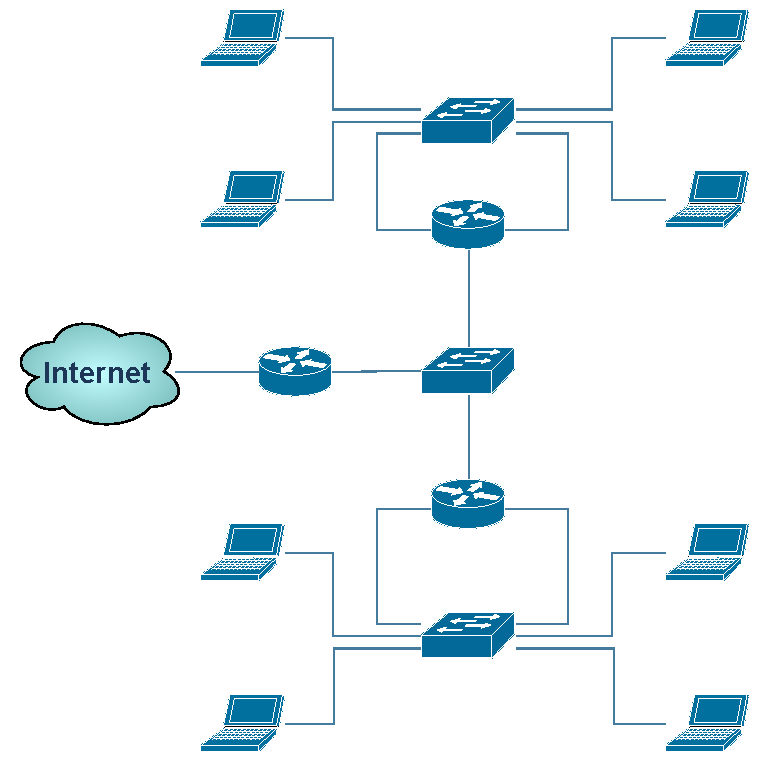
\includegraphics[]{network_structure.pdf}
    \caption{ネットワーク構造}
\end{figure}

実験で使用した端末はノートパソコンであり,インストールされていたOSはWindows,またはMacOSであった.
ただし,主に使用したOSはWindowsであり,更に今回の実験における操作では,Windows10とWindows11には決定的な動作の違いが見受けられなかったため,
Windows10,11をインストールしたノートパソコンを端末として扱うことにする.

\subsection{ネットワークアドレスの分割}
今回構築したネットワークにはネットワークアドレス,172.31.0.0/16が割り当てられた.
これをサブネット化することで,172.31.20.0/24,172.31.21.0/24,172.31.24.0/24,172.31.25.0/24の4つの子ネットワークに分割した.

\subsection{デバイスへのIPアドレスの付与}
\subsubsection{端末へのIPアドレスの付与}
WindowsコンピュータのIPアドレスの付与は「設定」→「ネットワークとインターネット」→「イーサネット」→「IP設定」などから手動で行うことができる.
付与するIPアドレスは172.31.21.0/24以外のネットワークでは一方の端末にはホスト部が2,もう一方には3となるIPアドレスを付与した.
172.31.21.0/24ではホスト部が4または5となるIPアドレスを付与した.
サブネットマスクにはWindowsの場合$2^{32}$ビットで表される値を指定する必要があり,255.255.255.0と入力した.
デフォルトゲートウェイはいづれのサブネットでもホスト部が1となるIPアドレスを指定した.
DNSサーバの設定では,工科大のDNSサーバのIPアドレスである172.30.0.2を指定した.

\begin{table}[h]
    \centering
    \begin{tabular}{|l|l|}
        \hline
        \rowcolor[gray]{0.9}
        項目 & 設定内容 \\ \hline \hline
        IPアドレス & ホスト部が2または3または4または5のIPアドレス \\ \hline
        サブネット プレフィックスの長さ & 255.255.255.0 \\ \hline
        ゲートウェイ & ホスト部が1のIPアドレス \\ \hline
        優先DNS & 172.30.0.2(工科大のDNSサーバ)\\ \hline
    \end{tabular}
    \caption{IP設定}
\end{table}

\subsubsection{スイッチ及びルーターの初期設定}
スイッチ及びルーターには外部の端末から遠隔ログインにより設定を行った.
これを容易に行えるようにPuttyという遠隔操作ツールを用いた.
使用したソフトウェアのバージョンはWindows-64bit x86のバージョン0.82である.

\subsubsection{スイッチ及びルーターへのIPアドレスの付与}


\subsection{ルーティング設定}

\section{考察}

\begin{thebibliography}{99}
    \bibitem{citekey} 須山敦志,「ベイズ推論による機械学習入門」,講談社,2017
    \bibitem{de:putty} 「Putty」 \url{https://www.chiark.greenend.org.uk/~sgtatham/putty/}
\end{thebibliography}

\end{document}